\cleardoublepage

\section{项目实施方案}

\subsection{软件需求分析}

本项目的目标是实现一个高效的工业场景导入和渲染系统,以下是针对关键需求的分析:

\par (1)系统需支持包含千万级多边形的工业模型导入,确保数据预处理过程在 1 小时内完成。内存占用不得超过 24 GB。这要求预处理算法的时间复杂度不超过 $O(N\log N)$,空间复杂度不超过 $O(N)$。必要时可考虑数据压缩技术,以进一步减少内存占用。

\par (2)在运行时,系统显存占用应不超过 8 GB,渲染帧率需稳定在 30 FPS 左右,以满足实时交互需求。系统应保持较高的画面质量,渲染结果与原始模型的视觉差异应控制在可接受范围内。这要求系统具备先进的 LOD 机制,在提高渲染性能的同时保证画面质量的稳定。流式加载需具备异步性,能够在不影响渲染性能和画面质量的同时,实现场景的动态加载。

\par (3)在帧率、显存占用、内存占用、预处理时间以及画面保真度等关键性能指标上,系统应至少达到与虚幻引擎 Nanite 相当的水平,并在部分指标上实现超越。这要求本项目尽可能探索 Nanite 因平台兼容性限制而未能采用的技术路线,如网格着色器、稀疏资源等先进的 Vulkan 特性。

\par (4)系统应具有较强的鲁棒性,能够适应不同类型的工业场景及 CAD 模型,并能根据不同硬件配置进行优化。因此,系统需选取多种不同类型的工业场景进行测试和优化。与此同时,系统需支持动态调整 LOD 选择与流式加载策略,确保在不同硬件环境下都能达到预期性能。

\subsection{项目整体架构}

\par 本项目的整体架构可分为预处理阶段与运行时阶段,如\autoref{fig:流程}所示。

预处理阶段主要负责对场景中的数据进行解析、处理和保存。具体包括将模型划分成簇、为模型生成 LOD、将场景数据组织成便于流式加载的形式等步骤。这些经过预处理的场景信息将被缓存在 CPU 内存中,为运行时的按需加载提供数据支撑。

\par 在运行时阶段,主要包括几何模块与流式加载模块两个核心部分。几何模块负责生成 G-Buffer\cite{lauritzen2010},为后续的光照计算提供基础几何信息。在任务着色器(Task Shader)中,不仅会以簇为单位进行 LOD 选择与可见性剔除,还会根据测试结果评估当前视角所需的几何数据,进而为流式加载模块提供调度指引。流式加载模块则依据几何模块的请求,将相应的场景数据按需加载至 GPU 显存。渲染管线的其余部分(如准备绘制指令、光照与后处理等)则由原有引擎提供。

\begin{figure}[htbp]
    \centering
    \includegraphics[width=\linewidth]{流程.png}
    \caption{\label{fig:流程}项目流程图}
\end{figure}

\par 综上所述,本项目在原有引擎渲染管线的基础上,主要负责对几何模块进行修改,新增流式加载模块,并在预处理阶段实现了将模型划分成簇与生成 LOD 的功能。通过这些改进,原渲染管线的性能得到了显著优化,帧率明显提升,显存占用有所降低,同时保持了良好的画面保真度。

\section{基于簇的 GPU 驱动渲染管线}

\subsection{引言}

GPU 驱动的渲染管线是一种由 GPU 完成大部分渲染任务的渲染架构,与传统的 CPU 驱动渲染管线相比,GPU 驱动渲染管线能够显著提高渲染效率,尤其在处理复杂大规模场景时。其核心思想是将大量渲染计算和数据处理任务交给 GPU 执行,充分利用 GPU 强大的并行计算能力,从而加速渲染过程。

本项目除了流式加载模块中涉及到 CPU 与 GPU 之间的通信外,其余渲染过程均在 GPU 上实现。与此同时,本项目引入了由任务着色器和网格着色器组成的新型渲染管线,代替了传统的计算着色器(Compute Shader)、顶点着色器(Vertex Shader)和几何着色器(Geometry Shader)的组合。网格着色器提出了“簇”这一新概念,通过将三角形组织为簇,显著提高了 GPU 批处理的性能\cite{Czubala2024}\cite{Santerre2020}。

\subsection{基于簇的渲染}

基于簇的渲染(Cluster-based Rendering)最早由育碧(Ubisoft)在游戏《刺客信条:大革命》(Assassin's Creed Unity)中提出\cite{Ubisoft2015}。该方法将最小的剔除单元从传统的实例(Instance)替换为簇。簇是由少量三角形组成的结构,一个实例通常包含多个簇。对于复杂模型,使用这种更加细粒度的剔除方式,能够更有效地减少需要绘制的多边形数量,从而显著降低渲染管线中的计算负担。

本项目在预处理阶段将模型划分成簇,并设计了基于簇的 GPU 驱动渲染管线,有效提高了渲染性能。

\subsubsection{簇的划分} \label{subsubsec:cluster division}

将模型划分成簇是预处理阶段的关键步骤之一,本项目使用了第三方库 MeshOptimizer 来实现这一过程\cite{meshoptimizer}。MeshOptimizer 是一个高效的网格优化库,提供了各种优化算法,可以有效地对网格进行简化和划分,从而提高 GPU 渲染的性能。

在具体实践中,本项目规定每个簇最多由 64 个顶点 和 124 个三角形组成。这样的划分方式有助于平衡簇的大小和渲染效率\cite{Kubisch2018}。

\subsubsection{基于簇的剔除} \label{subsubsec:cluster culling}

基于簇的剔除是在任务着色器中执行的,本项目目前实现的剔除算法包括视锥剔除(Frustum Culling)和圆锥剔除(Cone Culling)。

其中,视锥剔除是判断模型是否在相机视野范围内的一种剔除方法。在预处理阶段,本项目提前计算了每个簇的包围球(Bounding Sphere),通过在运行时测试该包围球与视锥体(View Frustum)的关系,来判断该簇是否位于当前相机视野范围内。如果包围球完全在视锥体外,则该簇可以被剔除,避免不必要的渲染计算。

圆锥剔除则是将簇中所有顶点的法线方向表达为一个圆锥,依此进行可见性判断。具体而言,如果相机的视角方向与圆锥范围内所有法线方向的点积均为负数,则说明该簇完全背对相机,可以整体剔除,不需要渲染。在预处理阶段,本项目预计算了每个簇对应的圆锥信息,包括圆锥的顶点、主轴方向和定角等,这些信息可以直接用于运行时的剔除操作。

\subsection{测试分析报告}

本项目实现了簇的可视化功能,并在多个场景中进行了测试,如\autoref{fig:Meshlet}所示。可以看出,簇划分的结果较为规整,能够较好地贴合几何结构,且不同场景下的可视化效果均展现出了良好的适应性和一致性。

% \begin{figure}[htbp]
%     \centering
%     \includegraphics[width=\linewidth]{Meshlet.png}
%     \caption{\label{fig:Meshlet}簇的可视化效果图}
% \end{figure}

\begin{figure*}[htbp]
    \centering

    \begin{subfigure}[b]{0.48\linewidth}
        \centering
        \includegraphics[width=\linewidth]{Meshlet.png}
        \caption{Sponza 场景}
    \end{subfigure}
    \hfill
    \begin{subfigure}[b]{0.48\linewidth}
        \centering
        \includegraphics[width=\linewidth]{factory_meshlet.png}
        \caption{Factory 场景}
    \end{subfigure}

    \caption{簇的可视化效果图}
    \vspace{-0.2cm}
    \label{fig:Meshlet}
\end{figure*}

与此同时,本项目在 Factory 场景下设置了固定相机轨迹进行测试,测量了不同剔除策略下的平均帧时间,以及 GPU 在裁剪阶段丢弃的平均图元数量。GPU 在裁剪阶段丢弃的图元数量越多,意味着处理了更多无效的几何数据;相反,若丢弃的图元数量越少,则表明所采用的剔除策略更加高效,能够在早期阶段排除无效数据,从而减少不必要的图形处理开销。具体测试结果见\autoref{tab:culling}。

\begin{table}[H]
    \caption{\label{tab:culling}不同剔除策略下的渲染性能测试结果}
    \begin{tabularx}{\linewidth}{|c|X<{\centering}|c|}
        \hline
        剔除策略 & GPU 在裁剪阶段丢弃的图元数 & 帧时间 \\ \hline
        不使用剔除 & 40713.9k & 240.7ms \\ \hline
        使用实例级剔除 & 40350.5k & 233.5ms \\ \hline
        使用视锥剔除 & 28557.5k & 147.9ms \\ \hline
        使用圆锥剔除 & 39249.1k & 230.7ms \\ \hline
        同时使用视锥剔除和圆锥剔除 & 27575.3k & 142.7ms \\ \hline
    \end{tabularx}
\end{table}

从表中数据可以看出,实例级的剔除对于工业大场景的性能提升有限,而基于簇的视锥剔除和圆锥剔除能够有效减少绘制三角形的数量。二者相结合的基于簇的剔除策略显著提升了渲染帧率,证明了基于簇的渲染方法在提高渲染效率方面的有效性。

\section{LOD 机制}

\subsection{引言}

LOD 技术指根据物体模型在显示环境中的重要度,决定物体渲染的资源分配。当物体在屏幕空间所占的像素较少时,说明该物体重要度偏低,可以使用较粗糙的细节层次。这种技术能在保证基本画面质量的同时,有效减少屏幕上绘制的三角形数量,提高渲染性能\cite{Deng2017}。而在本项目中,LOD 机制不仅用于提升渲染效率,还与流式加载相结合。对于重要度较低的物体,只加载其较粗糙的模型,以进一步降低显存占用。

\subsection{LOD生成} \label{subsec:LOD generation}

LOD 生成部分参考了 Nanite 的核心思想,采用了基于网格简化的 LOD 生成办法\cite{Jensen2023},但在具体实现上有所不同。整体过程大致可分为以下几步\cite{Xavier2024}:

\newcommand{\stepref}[1]{\textbf{Step~\ref{#1}}}

\begin{enumerate}
    \item 将初始模型划分为簇;
    \item 根据簇与簇之间的连接性,将簇组织成簇组(cluster group),每个簇组最多包含 16 个簇;
    \item 对每个簇组进行简化,确保每个簇组的边界完整,从而避免不同 LOD 之间出现裂缝;
    \item 将简化后的簇组重新划分为新的簇;
    \item 如果新的簇数量仍然过多,则返回步骤 2 进行进一步简化;否则结束生成过程。
\end{enumerate}

其中,步骤 1 已经在 \ref{subsubsec:cluster division} 节中,通过使用 MeshOptimizer 库得到了有效解决。步骤 4 也可以采用类似的方法来处理。

在步骤 2 中,本项目将生成的簇进一步划分为若干簇组。理想情况下,簇组之间的共享边应尽可能少,以最大程度减少后续简化过程中需要锁定的顶点数量。可将每个簇抽象为图中的一个节点,若两个簇之间存在共享边则连接一条边,从而将该问题等价转化为串行图划分(Serial Graph Partitioning)问题,进而采用 METIS 等图划分库进行高效求解\cite{METIS}。

对于每个簇组,将使用 MeshOptimizer 库对其进行锁定边界的简化,即步骤 3。简化结束后,MeshOptimizer 库会返回一个误差值,用以表示简化后的网格与原网格的相对误差。该误差值将在 \ref{subsec:run-time lod select} 节中用于运行时的 LOD 选择。

上述简化方法在处理完全连接的网格时表现良好,但对于具有很多互不相连小面的网格(faceted meshes),这种方法会失效。这是因为网格中相互连接的三角形数量不足,无法在不引入过多误差的前提下达到期望的简化比例。为了缓解上述情况,一种可行的方法是将空间中距离较近的顶点进行合并,帮助简化器去除更多的三角形,以推动简化过程。

为了高效查询每个顶点的最近邻,本项目使用 K-D 树对所有顶点进行管理\cite{bentley1975}。K-D 树构建的时间复杂度一般为 $O(N\log N)$,单次查询的时间复杂度为 $O(\log N)$。相比枚举算法的 $O(N^2)$ 时间复杂度,K-D 树的效率更高,满足本项目对预处理时间的需求。

此外,为避免顶点合并后模型的视觉差异过大,本项目在顶点合并时不仅考虑顶点在空间上的距离,还给予了纹理坐标、法向量等其他顶点属性适当的权重。

为进一步提高预处理速度,本项目引入 oneTBB 库对整个预处理过程进行多线程加速\cite{oneTBB},重点对顶点合并等易成为瓶颈的步骤进行了优化。

完成以上所有步骤后,不同 LOD 等级的簇将构成一个有向无环图(DAG),如\autoref{fig:DAG}所示\cite{WangXi2022}。该图中,每个节点表示一个簇,每个节点可能有多个父节点,父节点是由子节点简化得来的。被矩形框住的节点同属一个簇组。在随后的运行时阶段,本项目将基于该有向无环图进行 LOD 选择。

\begin{figure}[ht]
    \centering
    \includegraphics[width=\linewidth]{DAG.png}
    \caption{\label{fig:DAG}LOD的DAG示意图}
\end{figure}

\subsection{运行时 LOD 选择} \label{subsec:run-time lod select}

\par 为了在运行时进行 LOD 选择,必须对\autoref{fig:DAG}中的有向无环图进行遍历。而传统的遍历方法缺乏并发性,无法直接在 GPU 上执行。为了实现并行,本项目对每个节点(簇)独立进行 LOD 选择。为此,需要在 LOD 生成阶段预先维护每个节点(簇)所在簇组的误差值、包围球,以及其父节点所在簇组的误差值和包围球信息\cite{WangQian2016}。由于每个节点可能有多个父节点,且这些父节点可能属于不同的簇组,因此在维护父节点的误差值和包围球时,通常取其中的最大值。

在运行时,基于这些预计算的数据,本项目将计算每个节点自身在屏幕空间上的误差 $cluster\_error$,以及其父节点在屏幕空间上的误差 $parent\_error$。这两者的值由节点自身的误差以及其包围球在屏幕空间上的投影大小决定。与此同时,本项目设置了一个阈值 $lod\_threshold$,当且仅当 $cluster\_error < lod\_threshold$ 且 $parent\_error \geq lod\_threshold$ 时,该节点(簇)才有可能被绘制。这种可见性判定机制确保了渲染时的层级互斥性:当某个子节点满足条件被绘制时,其所有父节点必然不符合渲染条件,子节点和父节点不会被同时绘制。

这种基于簇的 LOD 选择方法不仅具有并行化优势,还可与基于簇的剔除(参见\ref{subsubsec:cluster culling})一同在任务着色器中完成,无需引入额外的渲染通道。该方案显著降低了代码实现的复杂度,同时提升了整体渲染效率。

\subsection{测试分析报告}

本项目首先基于 Sponza 场景的局部模型进行 LOD 生成测试,效果如\autoref{fig:LOD generation}所示。图中上方展示渲染结果,下方呈现对应的簇可视化效果。各 LOD 层级对应的顶点数、三角形数及簇数统计详见\autoref{tab:LOD}。

% \begin{figure}[!htb]
%     \centering
%     \includegraphics[width=\linewidth]{LOD生成.png}
%     \caption{\label{fig:LOD generation}各级 LOD 的生成效果图}
% \end{figure}

\begin{figure*}[h]
    \centering
    % 第一列(LOD 0)
    \begin{subfigure}[t]{0.32\linewidth}
        \centering
        \includegraphics[width=\linewidth,height=1.6in,keepaspectratio]{tiger0.png}\\
        \vspace{0.1cm}
        \includegraphics[width=\linewidth,height=1.6in,keepaspectratio]{tiger0_meshlet.png}
        \caption{LOD 0}
    \end{subfigure}%
    \hfill
    % 第二列(LOD 3)
    \begin{subfigure}[t]{0.32\linewidth}
        \centering
        \includegraphics[width=\linewidth,height=1.6in,keepaspectratio]{tiger3.png}\\
        \vspace{0.1cm}
        \includegraphics[width=\linewidth,height=1.6in,keepaspectratio]{tiger3_meshlet.png}
        \caption{LOD 3}
    \end{subfigure}%
    \hfill
    % 第三列(LOD 6)
    \begin{subfigure}[t]{0.32\linewidth}
        \centering
        \includegraphics[width=\linewidth,height=1.6in,keepaspectratio]{tiger6.png}\\
        \vspace{0.1cm}
        \includegraphics[width=\linewidth,height=1.6in,keepaspectratio]{tiger6_meshlet.png}
        \caption{LOD 6}
    \end{subfigure}
    \caption{各级 LOD 生成效果对比图}
    \label{fig:LOD generation}
\end{figure*}

\begin{table}[H]
    \caption{\label{tab:LOD}各级 LOD 对应的顶点数、三角形数和簇数}
    \begin{tabularx}{\linewidth}{|X<{\centering}|X<{\centering}|X<{\centering}|X<{\centering}|}
        \hline
        LOD级别 & 顶点数 & 三角数 & 簇数 \\ \hline
        LOD 0 & 5032 & 7128 & 80 \\ \hline
        LOD 3 & 2223 & 2997 & 36 \\ \hline
        LOD 6 & 1108 & 1264 & 18 \\ \hline
    \end{tabularx}
\end{table}

从上述结果可以看出,LOD 生成的核心功能基本实现,随着 LOD 级别的增大,顶点数、三角形数和簇数都有了明显下降,效果良好。

本项目对运行时 LOD 选择机制进行了验证测试,通过远景、中景和近景三个典型视距下的渲染效果对比,展示了 LOD 机制的实际运行表现(见\autoref{fig:LOD select})。图中第一行为原始场景渲染结果,第二行为应用 LOD 后的渲染结果,第三行通过色彩编码可视化 LOD 层级分布,其中蓝色表示最高精度的 LOD 0,紫色代表中间层级,红色则对应最简化的 LOD。

\begin{figure*}[h]
    \centering
    % 第一列(远景)
    \begin{subfigure}[b]{0.32\linewidth}
        \centering
        \includegraphics[width=\linewidth,height=1.6in,keepaspectratio]{远LOD0.png}\\
        \vspace{0.1cm}
        \includegraphics[width=\linewidth,height=1.6in,keepaspectratio]{远LOD.png}\\
        \vspace{0.1cm}
        \includegraphics[width=\linewidth,height=1.6in,keepaspectratio]{远LODv.png}
        \caption{远景}
    \end{subfigure}%
    \hfill % 确保子图之间有空隙
    % 第二列(中景)
    \begin{subfigure}[b]{0.32\linewidth}
        \centering
        \includegraphics[width=\linewidth,height=1.6in,keepaspectratio]{中LOD0.png}\\
        \vspace{0.1cm}
        \includegraphics[width=\linewidth,height=1.6in,keepaspectratio]{中LOD.png}\\
        \vspace{0.1cm}
        \includegraphics[width=\linewidth,height=1.6in,keepaspectratio]{中LODv.png}
        \caption{中景}
    \end{subfigure}%
    \hfill % 确保子图之间有空隙
    % 第三列(近景)
    \begin{subfigure}[b]{0.32\linewidth}
        \centering
        \includegraphics[width=\linewidth,height=1.6in,keepaspectratio]{近LOD0.png}\\
        \vspace{0.1cm}
        \includegraphics[width=\linewidth,height=1.6in,keepaspectratio]{近LOD.png}\\
        \vspace{0.1cm}
        \includegraphics[width=\linewidth,height=1.6in,keepaspectratio]{近LODv.png}
        \caption{近景}
    \end{subfigure}
    \caption{LOD 选择策略在不同视距下的应用效果}
    \label{fig:LOD select}
\end{figure*}

测试结果表明,本项目的 LOD 选择机制具有明确的视距相关性:在远景下,系统倾向于选择最粗糙的 LOD(红色区域);在中景下,中等细节层次的 LOD(紫色和蓝色区域)成为主导;在近景下,画面上基本采用最精细的 LOD(蓝色区域)。这种与视距高度匹配的 LOD 分布特征,充分验证了本项目 LOD 选择算法的合理性。

\section{流式加载} \label{sec:streaming}

\subsection{引言}

流式加载是一种基于用户需求的动态资源加载技术。与传统的预加载方式相比,该技术能够在运行时根据用户需要和显存使用情况,动态加载和释放资源,有效避免了一次性加载大规模数据带来的显存压力\cite{sahm2004}。

本项目的流式加载系统实现了双重优化机制:一是通过剔除技术,仅加载当前视野可见的场景数据\cite{CohenOr2003};二是结合 LOD 机制,对重要度较低的物体仅加载其较粗糙的模型数据。

在预处理阶段,本项目以簇组为单位存储场景数据,并将其按页缓存在 CPU 中;在运行时阶段,流式加载模块通过任务着色器传递的数据页信息,将需要加载的数据传输至 GPU 显存。这种设计在保证渲染性能和画面质量的前提下,实现了显存利用率的最大化。

\subsection{场景数据的存储}

在预处理阶段,本项目以簇组为单位对场景数据进行存储。主要原因是在任务着色器中,剔除计算与 LOD 选择本质上是以簇组为单位进行的。对于某一个簇组,要么整体渲染、要么整体跳过。在这种情况下,以簇组为单位存储数据具备以下优势:

\begin{enumerate}
    \item 降低 CPU 内存占用:若以簇为单位存储数据,由于簇与簇之间存在大量公共顶点,重复存储会导致内存占用大幅膨胀,而以簇组为单位能有效缓解该情况;
    \item 提高显存利用率:簇组内顶点与索引数据的紧凑布局有助于提高显存利用率,在有限的显存中存储更多有效几何信息;
    \item 提升访问效率:簇组结构具备更好的空间局部性\cite{MCCOOL2012},有助于提高缓存命中率,降低页表管理与数据交换的运行时开销。
\end{enumerate}

\subsection{动态加载}

在任务着色器中,所有簇组需依次进行剔除测试和 LOD 选择。只有通过测试簇组的几何数据会被加载至显存。任务着色器记录了所有通过测试簇组所对应的数据页编号,并将其传递给 CPU。CPU 利用页表(Page Table)对数据页进行统一管理,并借助 Vulkan 的稀疏资源机制,实现数据页的动态绑定,从而高效地完成资源调度。

\subsubsection{页表管理}

本项目中,页表对应的显存容量和数据页大小均为固定值,每个页表条目对应一个显存页。当 GPU 请求加载新的数据页时,CPU 首先检查该数据页是否已在页表中。若在,则不需要执行任何操作;若不在,则需在页表中寻找空闲条目,或选择一个当前帧未使用的数据页进行替换。页表结构如\autoref{fig:page table}所示。

\begin{figure}[htbp]
\centering
\includegraphics[width=\linewidth]{页表.png}
\caption{\label{fig:page table}页表示意图}
\end{figure}

目前本项目实现了两种数据页替换策略:一是随机替换策略,在页表已满的情况下,随机选取一个当前帧未使用的数据页换出;二是 LRU(最近最少使用)策略,优先换出最近使用频率最低的数据页。有关两种策略的性能对比将在 \ref{subsec:streaming test} 节中详细讨论。

极端场景下,若当前视角需要加载的场景数据过多,而页表没有空闲条目且页表中的数据页都已被当前帧使用,导致需要加载的数据页无法换入。这种情况下渲染缺乏数据支撑,场景中会出现“空洞”。为缓解该问题,本项目借鉴计算机网络中拥塞控制(Congestion Control)的思想\cite{Wiki-congestion},提出了根据页表压力动态调整 LOD 选择策略的方法。当页表压力过大时,可以提高 \ref{subsec:run-time lod select} 节中的 $lod\_threshold$,采用更激进的 LOD 选择策略:即便是在屏幕上占比较大的物体,也可能选择较粗糙的 LOD 版本。待页表压力缓解后,系统再逐步恢复原有的 LOD 选择标准。尽管该策略在一定程度上会降低画面质量,但能有效避免明显绘制错误的出现,提高流式加载过程的稳定性。

\subsubsection{稀疏资源}

稀疏资源是 Vulkan 1.2 集成的重要扩展,广泛应用于虚拟几何、虚拟纹理(Virtual Texture)等程序架构\cite{SparseResources}。传统的 Vulkan 资源需连续、完整地绑定至单一显存块,且绑定关系在资源的生命周期内不可修改。而稀疏资源突破了上述限制,允许资源分页绑定至多个显存页,并支持动态修改绑定关系,为高效的流式加载机制提供了强有力的支持。有关稀疏资源的详细机制和用法,本文在附录 \ref{appendix:sparse} 中做了进一步阐述。

本项目使用稀疏资源功能构建了一个逻辑上的大型缓冲区(Buffer),用于存储场景的所有几何数据。该缓冲区被划分为若干页,并绑定至多个独立的显存页。稀疏资源支持部分区域未绑定显存页,缓冲区的部分位置并不存在实际数据,因此该大型缓冲区的实际显存占用并不高。如\autoref{fig:page table}所示。

每当有新的数据页被换入页表中,CPU 会提交稀疏绑定命令,将页表条目对应的显存页绑定至缓冲区的目标区域。随后,CPU 再提交数据传输命令,将对应的场景数据复制到缓冲区中。

需要注意的是,Vulkan 对单个缓冲区的大小存在限制。因此,本项目将逻辑缓冲区划分成多个大小一致的物理缓冲区,并使用 Vulkan 的 Buffer Device Address 特性进行管理\cite{BDA}。在运行时阶段,为确保安全访问,系统仅允许网格着色器读取已加载数据的缓冲区区域,尽可能避免访问尚未绑定或尚未传输数据的空白区域。具体地,网格着色器可以根据当前簇组所在的数据页编号及其在数据页中的偏移量,准确计算其对应的缓冲区位置。

\subsubsection{异步加载}

为避免数据传输过程阻塞渲染流程,本项目采用了异步加载的策略\cite{UnityStreaming}。

本项目创建了独立的传输队列,用于执行数据上传任务,从而避免传输工作与执行绘制命令的图形队列发生竞争。与此同时,针对第 $i$ 帧所需的数据,系统并未在第 $i$ 帧内全部完成加载,而是延后至第 $i{+}1$ 帧渲染之前完成上传。这样可避免图形队列因等待传输队列而发生阻塞,提升了帧间的处理并行度。

理论上,在相机运动较为平稳的情况下,第 $i$ 帧需要的场景数据,大部分与第 $i{-}1$ 帧所需的场景数据重合,\ref{subsec:streaming test} 节的实验结果也证明了这一点。因此,即使复用第 $i{-}1$ 帧的几何数据,延迟一帧加载第 $i$ 帧的数据,对画面质量的影响微乎其微。但该方法显著提升了系统吞吐率和整体渲染效率,尤其适用于大规模场景下的流式加载需求。

\subsection{测试分析报告} \label{subsec:streaming test}

本项目使用了固定的相机轨迹,在 Factory 场景下测试了两种不同换页策略的性能。测试结果如\autoref{tab:swap page}所示。命中概率表示当前帧所需的数据页已在页表中的概率,页表耗时表示每帧维护页表所需的时间,绑定耗时表示每帧执行稀疏绑定操作所需的时间。

\begin{table}[H]
    \caption{\label{tab:swap page}不同换页策略的性能比较}
    \begin{tabularx}{\linewidth}{|X<{\centering}|X<{\centering}|X<{\centering}|X<{\centering}|X<{\centering}|}
        \hline
        换页策略 & 命中概率 & 页表耗时 & 绑定耗时 & 总耗时 \\ \hline
        随机替换 & 99.2\% & 2.86ms & 1.59ms & 4.45ms \\ \hline
        LRU & 99.2\% & 2.67ms & 1.47ms & 4.14ms \\ \hline
    \end{tabularx}
\end{table}

从表格数据可以看出,随机替换和 LRU 策略在命中概率上基本相同,性能差异主要体现在页表耗时和绑定耗时上。LRU 策略在页表维护和绑定过程中的耗时稍低,因此在后续测试中我们选择了性能更优的 LRU 策略。

此外,本项目还对数据页的大小进行了测试,以确定最佳的页大小,结果如\autoref{fig:page size}所示。

\begin{figure}[ht]
    \centering
    \includegraphics[width=\linewidth]{PageSize.png}
    \caption{\label{fig:page size}不同数据页大小对性能的影响}
\end{figure}

从测试结果可以看出,随着数据页大小的增大,命中概率逐渐提高,同时页表和绑定操作的耗时显著减少。当数据页大小过小时,由于页表容量保持不变,数据页数量较大,导致页表管理的开销上升,进而显著降低了页表的处理速度,同时稀疏绑定所消耗的时间也大幅增加。当数据页大小增大到 4096KB 时,由于页表容量有限,显存利用率下降,页表的压力增大,系统不得不采用更为激进的 LOD 选择策略,导致画面质量明显下降。因此,综合考虑性能和显存利用率,本项目最终选择了 2048KB 作为最优的数据页大小。

\section{项目成果}

\subsection{最终实验结果及分析}

本项目分别对 Sponza、Factory 两个场景进行了最终测试。两个场景的参数如\autoref{tab:scene}所示。

\begin{table}[H]
    \caption{\label{tab:scene}测试场景信息}
    \begin{tabularx}{\linewidth}{|X<{\centering}|X<{\centering}|X<{\centering}|c|}
        \hline
        场景 & 顶点数 & 三角形数 & 场景文件大小(.gltf)\\ \hline
        Sponza & 190,448 & 262,241 & 81.9 MB \\ \hline
        Factory & 140,875,512 & 46,958,504 & 3.6 GB \\ \hline
    \end{tabularx}
\end{table}

在性能测试中,本测试分别在启用与未启用 LOD 和流式加载功能的情况下,测量了预处理时间、显存占用、帧时间等关键性能指标。测试结果分别列于\autoref{tab:Sponza data}和\autoref{tab:Factory data}中,最终的运行效果对比如\autoref{fig:Sponza fig}和\autoref{fig:Factory fig}所示。

\begin{table}[H]
    \caption{\label{tab:Sponza data}Sponza 场景运行参数}
    \begin{tabularx}{\linewidth}{|X<{\centering}|X<{\centering}|X<{\centering}|X<{\centering}|X<{\centering}|}
        \hline
        ~ & 预处理时间 & 显存占用 & GPU 时间 & 帧时间 \\ \hline
        不开启 LOD 和流式加载 & 0.2s & 8.0MB & 0.8ms & 1.0ms \\ \hline
        开启 LOD 和流式加载 & 1.8s & 34.5MB & 0.9ms & 1.0ms \\ \hline
    \end{tabularx}
\end{table}

\begin{figure*}[htbp]
    \centering
    % 第一列(远景)
    \begin{subfigure}[b]{0.48\linewidth}
        \centering
        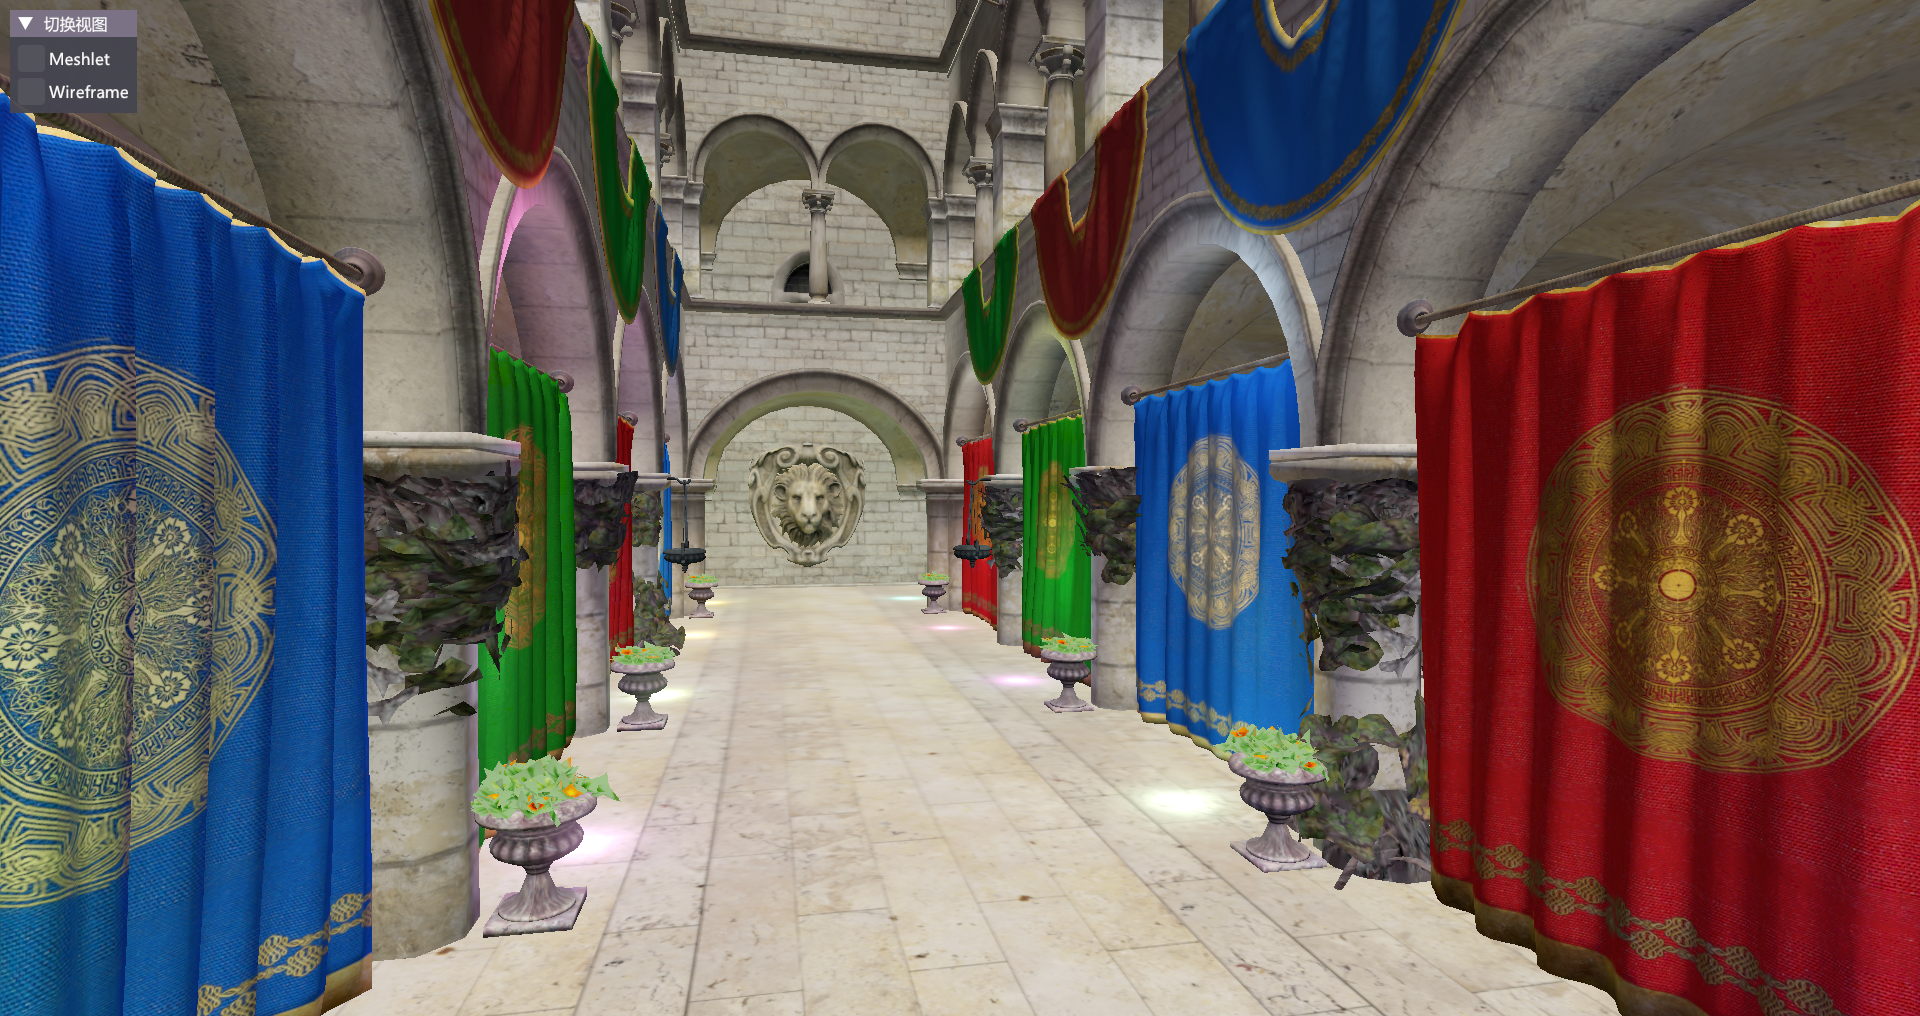
\includegraphics[width=2.9in]{Sponza0.png}
        \caption{不开启 LOD 和流式加载}
    \end{subfigure}%
    \hfill % 确保子图之间有空隙
    % 第二列(中景)
    \begin{subfigure}[b]{0.48\linewidth}
        \centering
        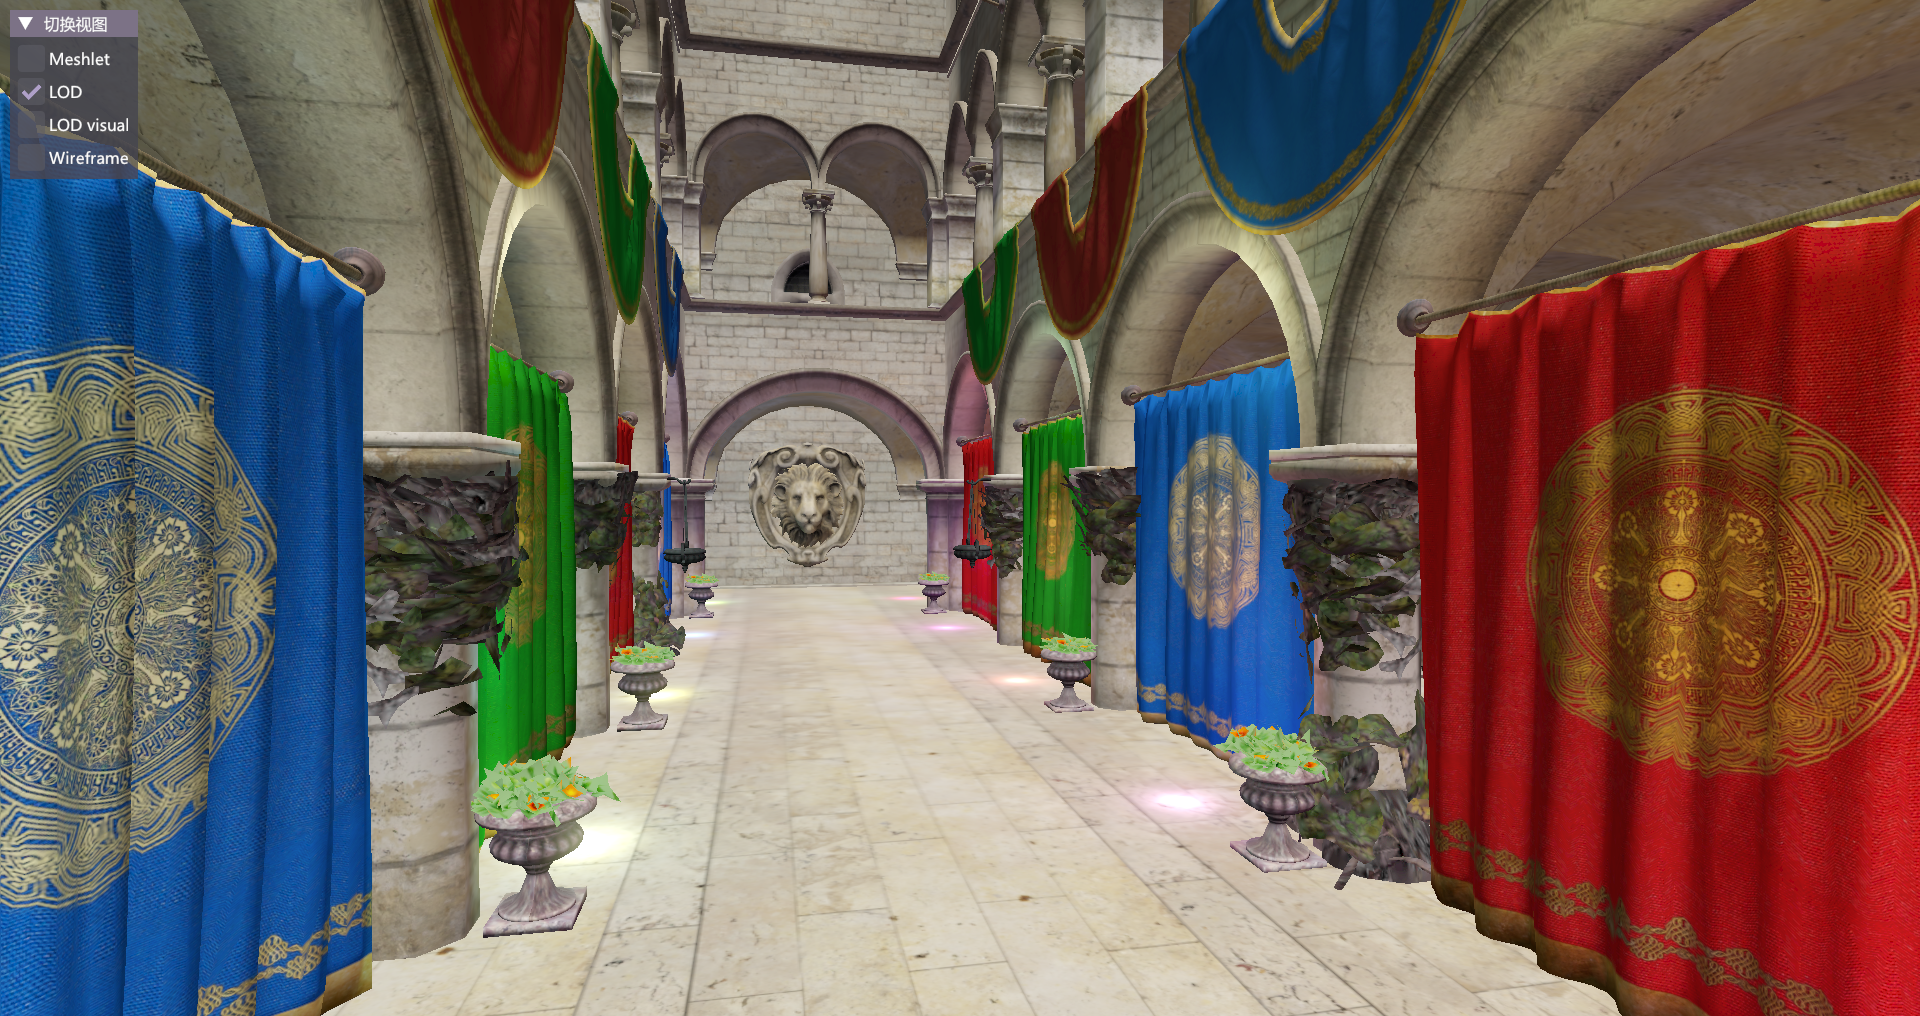
\includegraphics[width=2.9in]{Sponza1.png}
        \caption{开启 LOD 和流式加载}
    \end{subfigure}%
    \caption{Sponza 场景运行效果对比图}
    \vspace{-0.2cm}
    \label{fig:Sponza fig}
\end{figure*}

\begin{table}[H]
    \caption{\label{tab:Factory data}Factory 场景运行参数}
    \begin{tabularx}{\linewidth}{|X<{\centering}|X<{\centering}|X<{\centering}|X<{\centering}|X<{\centering}|}
        \hline
        ~ & 预处理时间 & 显存占用 & GPU 时间 & 帧时间 \\ \hline
        不开启 LOD 和流式加载 & 61s & 5.2GB & 230.3ms & 231.9ms \\ \hline
        开启 LOD 和流式加载 & 1480s & 5.1GB & 38.2ms & 38.5ms \\ \hline
    \end{tabularx}
\end{table}

\begin{figure*}[htbp]
    \centering
    % 第一列(远景)
    \begin{subfigure}[b]{0.48\linewidth}
        \centering
        \includegraphics[width=2.9in]{factory0.png}
        \caption{不开启 LOD 和流式加载}
    \end{subfigure}%
    \hfill % 确保子图之间有空隙
    % 第二列(中景)
    \begin{subfigure}[b]{0.48\linewidth}
        \centering
        \includegraphics[width=2.9in]{factory1.png}
        \caption{开启 LOD 和流式加载}
    \end{subfigure}%
    \caption{Factory 场景运行效果对比图}
    \vspace{-0.2cm}
    \label{fig:Factory fig}
\end{figure*}

从实验结果可以看出,对于简单场景(如 Sponza),LOD 与流式加载带来的性能收益较为有限;而在复杂工业场景(如 Factory)中,这些优化措施显著提升了渲染性能。帧率从不足 5 FPS 提升至约 25 FPS,实现了接近 5 倍的加速,基本满足实时交互需求。与此同时,开启流式加载后 GPU 时间与整体帧时间相近,说明虽然流式加载模块中存在 CPU 与 GPU 之间的数据交互,但并未造成明显的 CPU 负担,系统整体处于良好的负载均衡状态。

理论上在开启 LOD 后,由于每个模型新增了多个细节层次,显存占用应显著增加。然而,得益于流式加载机制的引入,系统仅加载当前视野所需的场景数据,从而有效地控制了数据加载的规模。由\autoref{tab:Factory data}可以看出,对于 Factory 场景,尽管开启了 LOD,显存占用却基本保持不变甚至有所下降。

本项目在画面质量上仍存在一些问题。如\autoref{fig:Factory fig}所示,开启 LOD 后画面出现明显瑕疵(Artifacts),左下角的柱子处尤为明显。经初步分析,产生瑕疵的原因主要是预处理过程中的顶点合并操作未充分考虑法向量因素,导致法向量精度下降,进而在光照计算中出现较大误差。后续需进一步改进法向量处理策略,尽可能提升画面质量。

与此同时,启用 LOD 与流式加载功能后,预处理时间显著增加。对于千万级多边形的模型,预处理时间可达 25 分钟左右。为避免用户在每次使用引擎时都重复执行预处理过程,本项目将预处理后的数据通过可持久化存储保存至磁盘中\cite{cereal}。此举显著提升了系统的启动速度,以方便在后续运行中快速加载和复用。

\subsection{工作总结}

首先,本项目成功实现了基于簇的 GPU 驱动渲染管线:在预处理阶段实现了簇的划分,在任务着色器中实现了两种不同的剔除策略,并构建了以网格着色器为核心的新型渲染管线。与此同时,本项目还实现了簇的可视化功能,为后续分析和优化工作奠定了坚实基础。

其次,项目引入了先进的 LOD 机制。在预处理阶段能够较为高效地自动生成 LOD,在运行时可动态调整渲染物体的 LOD,兼顾画质与性能。开启 LOD 后,在大规模工业场景中的性能提升最高可达约 5 倍。

最后,项目设计并实现了高效的流式加载机制。在预处理阶段将场景数据划分成页,并在运行结合页表进行调度管理。同时,借助稀疏资源这一技术路径,本项目能够管理远超显存容量的大型缓冲区,以实现虚拟几何技术。开启流式加载后,在场景数据规模超过显存容量的情况下,系统依然可以导入和渲染。

总体而言,本项目为大规模高精度工业场景的实时渲染提供了切实可行的技术路径,并为今后在该领域的进一步研究与应用奠定了坚实基础。

\subsection{未来展望}

尽管本项目在大规模工业场景的导入和实时渲染方面已取得初步成果,但距离实际工程应用仍存在一定差距。未来的改进方向主要包括:

\begin{itemize}
    \item \textbf{添加阴影支持}:由于系统改动了场景的存储结构,原引擎的阴影算法无法直接应用,需自行设计一种适配当前场景结构的阴影算法。未来可参考虚幻引擎中的虚拟阴影贴图(Virtual Shadow Map, VSM)思路\cite{VSM},实现高效的阴影算法。

    \item \textbf{实现高效的遮挡剔除}:目前管线只支持视锥剔除和圆锥剔除,缺乏高效的遮挡剔除(Occlusion Culling)机制。未来可引入遮挡查询技术,剔除更多不需要渲染的多边形,进一步释放性能\cite{coorg1997};

    \item \textbf{支持多材质系统}:当前渲染管线只支持单一材质的渲染。未来可以参考延迟材质(Deferred Material)的思想,实现一个可见性缓冲区(Visibility Buffer),来支持多个材质的同时渲染\cite{burns2013};

    \item \textbf{实现场景数据编码与解码}:当前系统的内存占用和显存占用依然较高,后续可以实现高效的数据编码和解码技术。在预处理阶段对场景数据进行编码,进一步压缩场景大小,可以显著降低显存、内存乃至磁盘空间的使用\cite{Mlakar2024}。同时,还需在 GPU 上实现高效的解码算法,保证渲染性能不受影响。
\end{itemize}

上述改进将进一步提升本项目在大规模工业场景中的数据处理能力、实时渲染能力和视觉表现力,为其在工程可视化、数字孪生等实际应用中奠定更广泛的技术基础。